\section{Motivation}

(For Ole Jakob) - General outline for motivation
\begin{enumerate}
    \item DAS and Big Data Processing
    \item CGF (Tools and Resources)
    \item Anomaly Detection and Unsupervised Learning
    \item Developing scalable applications
\end{enumerate}

\acrfull{das} is a rather new technology that allows for real-time analysis over fiber-optical cables. This technology has gained more recognition within the last decade, and due to their high sensitivity, \acrshort{das} systems are capable of detecting subtle environmental changes and anomalies. Analyzing these irregularities is a common and crucial task in various fields, and can be applied to tasks spanning landslide and earthquake detection to railroad and maritime monitoring. The ability to process and interpret \acrshort{das} data effectively is essential for extracting meaningful insights from these complex measurements. \\

\begin{figure}[!h]
    \centering
    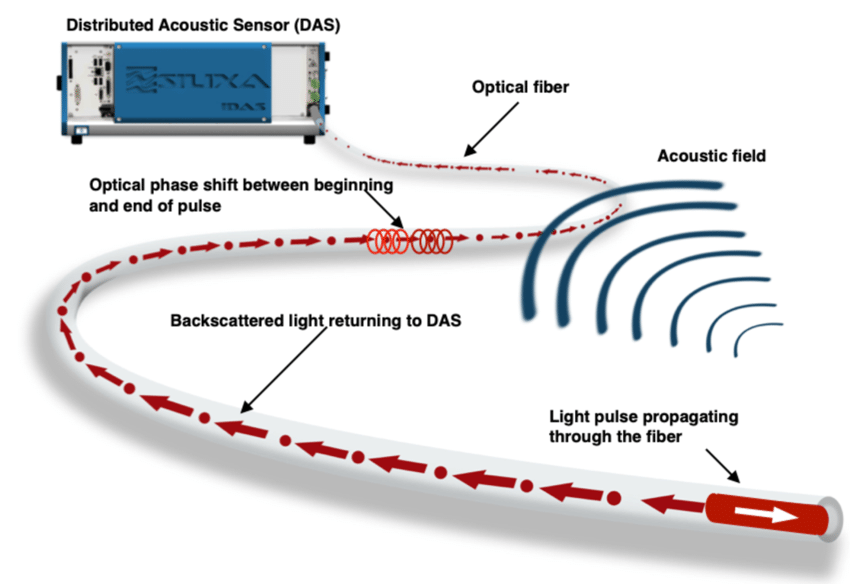
\includegraphics[width=0.7\linewidth]{figures/das.png}
    \caption{Showcase of how \acrshort{das} signals are recorded}
    \label{fig:das-fig}
\end{figure}


Recorded \acrshort{das} data has the potential to become quite large up to several terrabytes per experiment, underlying the importance of efficient algorithm design and processing techniques. Generally, languages such as Python and MatLAB are used for DAS analysis, due to their framework for data science applications. However, these programming languages are not designed for data intensive applications without having to leverage languages as C. Julia is a more novel language aimed at both data science and in general \acrfull{hpc} applications, and could prove really powerful as an alternative to existent program.


\subsection{DAS research at \acrshort{cgf}}

\acrfull{cgf} spend a lot of time and resources on processing and analysing \acrshort{das} data. Current tools for processing are quite slow, and do not utilize parallelization techniques that has the potential to drastically speed up computations. Additionally, analysis is often done using more traditional signal processing techniques, not leveraging the potential benefits of more novel \acrshort{ann} methods. \\ \\  


\subsection{Anomaly Detection for \acrshort{das} data}

Traditionally, clustering based \acrfull{ml} techniques such as K-MEANS, DBSCAN and HDBSCAN have been quite popular for anomaly detection. However, these methods often require manual feature engineering, require labeled datasets or generally do not scale to large datasets. 

\begin{figure}[ht]
    \centering
    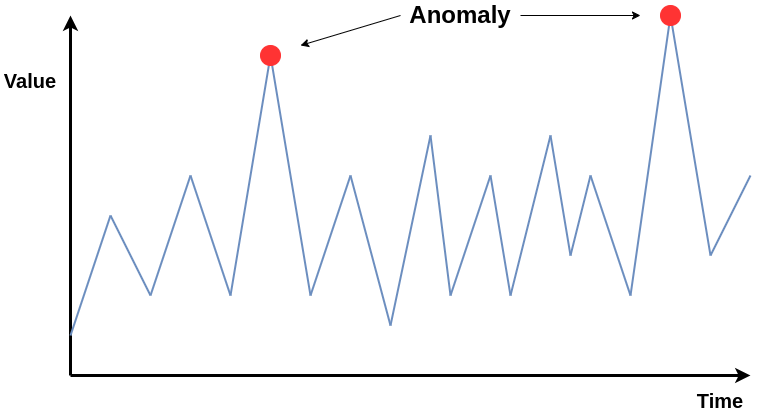
\includegraphics[scale=0.4]{figures/anolay_line.png}
    \caption{Example of anomalies in a dataset}
    \label{fig:anomaly_example}
\end{figure}


However, with the upcoming of \acrshort{das}, both unsupervised and supervised \acrfull{dl} methods have proven to produce even better results for anomaly detection. For \acrshort{das} data specifically, both scalability and manual labeling can become quite tedious, or outright non-feasible. For 

Unsupervised learning has in later years returned after the explosion of generative models [CITE]. Compared to their supervised alternatives, unsupervised do not require manual labeling. They're therefore not prone to some of the more common problems within supervised methods, such as detecting irregular events.   are well suited for detecting novel anomalies \cite{wei2022lstmautoencoder, srivastava2016unsupervised} compared to its supervised alternatives, and do not require manual labeling. This makes them 

Current autoencoder based approaches to anomaly detection of \acrshort{das} do not emphasize the overall memory consumption as well as the convertion of models to a real-time environment. This 

\acrshort{das} technology in itself has now started garnering attention for research, and several papers have previously studied  how one can process this data. \acrshort{ai} and \acrshort{ml} models have been constructed for looking at time series data, and analyzing sensor data, although several of theses have studied .  Only recently has \acrshort{ai}

Previous work on this data \cite{projthesis} revolved around processing \acrshort{hdf5} files as fast and efficient as possible, trying to parallellize already existent code, and take advantage of newer technologies, such as Julia.


We hereby present two programs: Judas and TinyDAS. Judas is a package consisting of methods for parsing \acrshort{das} data stored in \acrfull{hdf5} files,  processing them in a parallel manner. TinyDAS is a Python program for training autoencoder models and detecting anomalies , with a potential for real-time analysis. Combined, these two packages aims at expanding current tools available at \acrshort{cgf} for processing and analysing \acrshort{das} data. To evaluate our work, we use both proprietary and open source data. 

\begin{figure}[h]
    \centering
    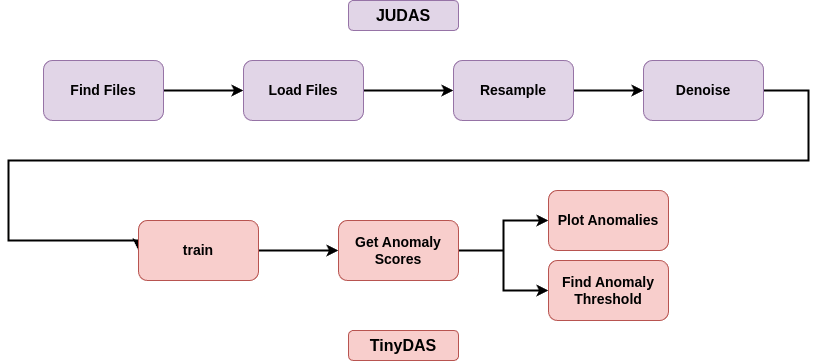
\includegraphics[scale=.5]{figures/api_overview.png}
    \caption{Judas and TinyDAS combined methodflow}
    \label{fig:judasnet_overview}
\end{figure}